\documentclass[border=8pt]{standalone}
\usepackage{tikz}
\definecolor{bg}{HTML}{171D2B}
\definecolor{acc}{HTML}{F7B538}
\begin{document}
\pagecolor{bg}
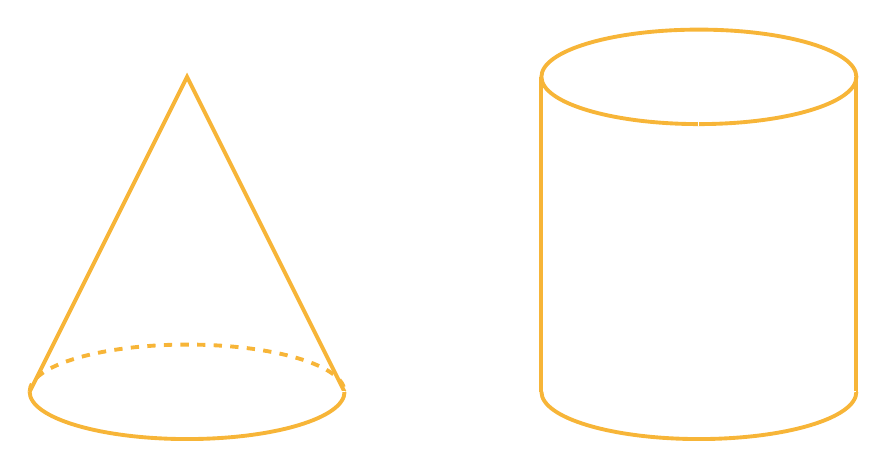
\begin{tikzpicture}[line width=1.4pt, text=white]
  % ===== Kerucut =====
  \draw[acc] (-2,0) -- (0,4) -- (2,0);
  \draw[acc] (-2,0) arc[start angle=180, end angle=360, x radius=2, y radius=0.6];
  \draw[acc,dashed] (-2,0) arc[start angle=180, end angle=0, x radius=2, y radius=0.6];
  \draw[white, dashed, thin] (0,0) -- (2,0);
  \draw[white, dashed, thin] (0,0) -- (0,4);
  \draw[white] (0,0.22) -| (0.22,0);
  \node[right] at (1.2,0.2) {$r$};
  \node[above left] at (0,1.8) {$t$};
  \node[above right] at (1.15,2.15) {$s$};
  % ===== Silinder =====
  \begin{scope}[xshift=6.5cm]
    \draw[acc] (-2,0) arc[start angle=180, end angle=360, x radius=2, y radius=0.6];
    \draw[acc] (-2,0) -- (-2,4);
    \draw[acc] (2,0) -- (2,4);
    \draw[acc] (0,4) ellipse (2 and 0.6);
    \draw[white, dashed, thin] (0,0) -- (2,0);
    \draw[white, dashed, thin] (0,0) -- (0,4);
    \draw[white] (0,0.22) -| (0.22,0);
    \node[right] at (1.2,0.2) {$r$};
    \node[above left] at (0,2) {$t$};
  \end{scope}
\end{tikzpicture}
\end{document}
